% =====================================================================
% Chapter 6 -- Experiments and Results
%
% Outline: outlines/ch6_experiments.md (approved 2026-10-22).
% Numbers: thesis/tables/*.csv and the generated tables (scripts/run_all.py); the
% source file is named in a comment where a number appears in the text.
% Switched to the reruns of October 2026 on 2026-10-26 (thesis_notes.md §1, §4).
% Every paragraph marked CLAUDE-DRAFT is to be rewritten by the author.
% =====================================================================

\chapter{Experiments and Results}
\label{chap:experiments}

% CLAUDE-DRAFT
This chapter reports the experiments with which we answer the research question.
\Cref{sec:exp-setup} gives the setup: the experiments, the data settings, the values of all parameters and the metrics.
The following sections present the experiments, each with its results and its conclusion.

% ---------------------------------------------------------------------
\section{Experimental Setup}
\label{sec:exp-setup}

% CLAUDE-DRAFT
\Cref{tab:ch6_experiments} lists the experiments and the objective of \cref{sec:intro-rq} that each addresses.
Each consists of runs of the protocol of \cref{alg:protocol} that differ in one factor: the strategy, the LoRA rank, the number of training volumes or of updates per task, the task order, the use of replay or of gradient scaling.
The pretrained model is the reference in every experiment, and joint fine-tuning is the upper reference for the comparison of the strategies and for the amount of labelled data.
A diagnostic experiment with task-specific LoRA trained on patellar cartilage alone tests why this strategy did not learn that structure in the task sequence (\cref{sec:exp-patellar}).
In total, we report 38 runs.
\Cref{sec:app-matrices} gives the evaluation matrices of all of them.
% source: results/experiment_index.csv, runs with a role other than "excluded" (29 sequence runs + 4 joint runs + 5 single-task diagnosis runs)

\subsection{Task Orders and Few-Shot Settings}
\label{subsec:exp-data}

% CLAUDE-DRAFT
In the original task order, the structures are trained in the sequence lateral tibial cartilage, medial tibial cartilage, femoral cartilage, patellar cartilage, medial meniscus and lateral meniscus.
We chose this order at random.
The second order is its reverse.
Sequential fine-tuning, task-specific LoRA and shared LoRA were trained in both orders.
We trained no further orders, because each would require a complete run of every strategy.

\begin{table}[tb] % after the first paragraph of 6.1.1: a top float cannot go on the chapter's opening page
\centering
% CLAUDE-DRAFT
\caption[Overview of the experiments]{Overview of the experiments. Training volumes per task: 108 is the full training split. Objective: number of the research objective in \cref{sec:intro-rq}. All runs use the original task order unless stated otherwise.}
\label{tab:ch6_experiments}
% Generated by scripts/make_setup_tables.py. Do not edit.
\small\setlength{\tabcolsep}{4pt}
\begin{tabularx}{\linewidth}{@{}>{\raggedright\arraybackslash}p{3.1cm}>{\raggedright\arraybackslash}X >{\raggedright\arraybackslash}p{1.9cm} c c@{}}
\toprule
Experiment & Strategies and configurations & Training volumes per task & Objective & Section \\
\midrule
Comparison of the strategies & Seq. fine-tuning; Task-specific LoRA ($r = 4$); Shared LoRA ($r = 1024$) with and without replay; Prompt tuning; Distillation-based & 108 & 2 & \ref{sec:exp-main} \\
Upper reference: joint fine-tuning & Joint fine-tuning & 5, 10, 20, 108 & 2, 3 & \ref{sec:exp-main} \\
Diagnosis of the patellar failure & Task-specific LoRA ($r = 4, 16$) on patellar cartilage only; rank, learning rate, seed or epochs varied & 108 & 2 & \ref{sec:exp-patellar} \\
Amount of labelled data & Seq. fine-tuning; Task-specific LoRA ($r = 4$); Shared LoRA ($r = 1024$); each also with $k = 5$ and 216 epochs per task & 5, 10, 20, 108 & 3 & \ref{sec:exp-few-shot} \\
LoRA rank & Task-specific LoRA ($r = 4, 8$); Shared LoRA ($r = 4, 32, 128, 256, 512, 1024, 2048$) & 108 & 4 & \ref{sec:exp-rank} \\
Task order & Seq. fine-tuning; Task-specific LoRA ($r = 4$); Shared LoRA ($r = 1024$); each in original and reverse order & 108 & 4 & \ref{sec:exp-task-order} \\
\bottomrule
\end{tabularx}

\end{table}

% CLAUDE-DRAFT
With $k = 5$, 10 or 20 volumes per task (\cref{sec:data-splits,sec:app-volumes}) and $E = 10$ epochs, a task receives 50, 100 or 200 updates instead of 1{,}080 with the full training split.
The equal-updates runs train sequential fine-tuning, task-specific LoRA and shared LoRA with $k = 5$ and $E = 216$ epochs, which gives these 1{,}080 updates.
We ran them only for $k = 5$, the setting with the largest difference in updates.
Joint fine-tuning was trained on the same $k$ volumes, each with all six text prompts, that is, on $6k$ samples in a single stage.
% source: code/src/data/datamodule.py:41 (joint training concatenates the per-task splits); thesis/data_description.tex (all six tasks use the same k volumes)

\subsection{Training and Evaluation Configuration}
\label{subsec:exp-config}

% CLAUDE-DRAFT
\Cref{sec:app-params} lists the settings that all runs share and the parameters of each strategy.
The optimiser, the initial learning rate $\eta_0 = 10^{-4}$ and the fraction of foreground-centred patches follow the pretraining of VoxTell~\cite[Suppl.~Sec.~A]{rokuss2025voxtellfreetextpromptableuniversal}.
The paper does not state the momentum, the weight decay or the learning-rate schedule.
For momentum and weight decay, we use the defaults of nnU-Net, on which VoxTell builds, and for the schedule a linear decay, close to nnU-Net's polynomial decay with exponent 0.9.\todo{cite: nnU-Net v2 code, nnUNetTrainer defaults (momentum 0.99, Nesterov, weight decay 3e-5, polynomial decay with exponent 0.9)}

% CLAUDE-DRAFT
Each run was trained on one NVIDIA A100 GPU with 40\,GB of memory on a cluster where a job may run for at most 24 hours.
We train each task for $E = 10$ epochs so that most runs with the full training split take about one such job (\cref{sec:exp-compute}).
\Cref{sec:app-params} gives the software versions and describes how runs that reached this limit were continued.

% CLAUDE-DRAFT
For the comparison of the strategies, we use rank $r = 4$ for task-specific LoRA and $r = 1024$ for shared LoRA.
We chose these ranks from the test results of the rank experiment, for the reasons given in \cref{sec:exp-rank}.
The choice therefore favours the two LoRA configurations in the comparison, and we report the run with $r = 8$ for task-specific LoRA as well, so that the alternative is visible.\todo{defense: main-comparison ranks chosen on test-split results (optimistic bias)}

\subsection{Metrics and Statistical Analysis}
\label{subsec:exp-metrics}

% CLAUDE-DRAFT
We report the five metrics of \cref{sec:bg-metrics}.
Adaptation, Final Forgetting and the control-task drop are primary, because the research question asks how the strategies trade adaptation against forgetting of earlier tasks and of pretrained ability.
Final Performance and Transfer are secondary.
We do not report ZSCL's third metric, Avg., the mean over all entries of stages 1 to~$T$~\cite[Sec.~4]{zheng2023preventingzeroshottransferdegradation}, because it combines adaptation, retention and transfer, which we analyse separately.

% CLAUDE-DRAFT
For task-specific LoRA, the control-task drop is zero and Final Forgetting is near zero by construction (\cref{subsec:method-lora}), so its comparison rests on Adaptation and Final Performance.
% values: thesis_notes.md section 2 (task-specific LoRA Final Forgetting per run, checked 2026-11-01)
For joint fine-tuning, which has no task sequence, only Final Performance and the control-task drop are defined.
All metrics are computed from mean \gls{dsc} fractions and reported with three decimals.
Single entries of the evaluation matrices are given with two decimals, as in the figures; \cref{sec:app-matrices} gives them with three.

% CLAUDE-DRAFT
Each configuration was trained once, so we cannot estimate how results vary with the training randomness or with the choice of training volumes.
The only variability we can estimate is that over the test volumes, and we do so with a bootstrap~\cite{efron1993bootstrap}.
In each of $N_{\mathrm{boot}} = 2000$ draws, the 24 SKM-TEA test volumes are resampled with replacement, the same draw is used for all tasks and all stages, and the 4 control-task volumes are resampled separately.
Every metric is then recomputed from the resampled means.
% source: scripts/compute_cl_metrics.py (N_BOOTSTRAP = 2000; seed per run and evaluation derived from BOOTSTRAP_SEED = 0)
We report the 2.5 and 97.5 percentiles of the resampled values as a 95\,\% interval.
The figures show these intervals, and the tables show only the values on the full test set; in the text, single-run intervals are given only for the patellar diagnosis (\cref{sec:exp-patellar}).
With only 4 control-task volumes, the intervals of the control-task drop are coarse.

% CLAUDE-DRAFT
All runs are evaluated on the same test volumes, so the results of two runs are correlated, and overlapping intervals do not show that two runs perform alike.
For the difference between two runs, we therefore apply the same draws to both runs and compute the interval of the difference (paired bootstrap).
In the text, we give these intervals where a statement depends on them, that is, for small differences and for differences we describe as absent.
All other reported differences have intervals that exclude zero by a wide margin.
% source: all dropped intervals checked 2026-11-04 (cl_differences.csv): none contains zero; the full intervals of every compared pair are in cl_differences.csv
% source: scripts/compare_strategies.py (one set of N_BOOTSTRAP index draws applied to both runs of a pair)
We interpret these intervals only for the comparisons that the experiments were designed for, which set a strategy against sequential fine-tuning or joint fine-tuning, or a run against the run that differs from it only in the factor studied (\cref{tab:ch6_experiments}).
% checked 2026-11-04: all 18 sentences with paired intervals in Ch. 6 compare a CL strategy vs seq. FT, a run vs its counterpart differing only in the studied factor (order, volumes/updates, replay, scaling, evaluated checkpoint), or joint FT vs strategies with the same volumes
Other differences, such as those between two continual-learning strategies or between LoRA ranks, are reported without intervals.
The intervals are not corrected for the number of comparisons, so we use them to describe differences, not to test them, and call no difference significant.

% ---------------------------------------------------------------------
% Weight ensemble and gradient scaling are reported in Sec. 6.3 (split 2026-11-02; replay back in 6.2 since 2026-11-04); the checkpoint rule stays here.
\section{Comparison of the Strategies}
\label{sec:exp-main}
% Rewritten 2026-10-26 for the reruns; readings follow the author's decisions Q1-Q9 (thesis_notes.md §1, 2026-10-26).

% CLAUDE-DRAFT
This experiment asks how the six strategies trade adaptation against forgetting when each task is trained on the full training split in the original task order, with joint fine-tuning as the upper reference (\cref{tab:ch6_experiments}).
\Cref{tab:ch6_main} gives all metrics, \cref{fig:ch6_main_metrics} shows them with their bootstrap intervals, and \cref{fig:ch6_main_matrices} shows the evaluation matrices from which they are computed.

\begin{table}[tb]
\centering
% CLAUDE-DRAFT
\caption[Results of the comparison of the strategies]{Results of the comparison of the strategies (full training split, original task order, one run each). Mean \gls{dsc}; $\uparrow$/$\downarrow$: higher/lower is better. Bold: best of the six strategies in each column. $^{\dagger}$: zero or near zero by construction (\cref{subsec:method-lora}), not ranked. --: not defined for joint fine-tuning.}
\label{tab:ch6_main}
% Generated by scripts/make_results_tables.py from thesis/tables/cl_metrics.csv. Do not edit.
\small\setlength{\tabcolsep}{4pt}
\begin{tabular}{lrrrrr}
\toprule
Strategy & Adapt.\,$\uparrow$ & Forg.\,$\downarrow$ & Ctrl.\ drop\,$\downarrow$ & Final\,$\uparrow$ & Transf.\,$\uparrow$ \\
\midrule
Seq. fine-tuning & 0.717 & 0.704 & 0.979 & 0.130 & 0.001 \\
Task-specific LoRA ($r=4$) & 0.485 & 0.000 & 0.000 & 0.485 & 0.129 \\
Shared LoRA ($r=1024$) & 0.471 & 0.289 & 0.237 & 0.233 & 0.174 \\
Prompt tuning & 0.608 & 0.568 & 0.979 & 0.135 & 0.043 \\
Distillation-based & 0.744 & 0.732 & 0.979 & 0.134 & 0.002 \\
\midrule
Shared LoRA + replay ($r=1024$)$^{*}$ & 0.429 & 0.039 & 0.007 & 0.446 & 0.148 \\
\midrule
Pretrained model & 0.114 & 0.000 & 0.000 & 0.114 & 0.137 \\
\bottomrule
\end{tabular}

\end{table}

\begin{figure}[tb]
\centering
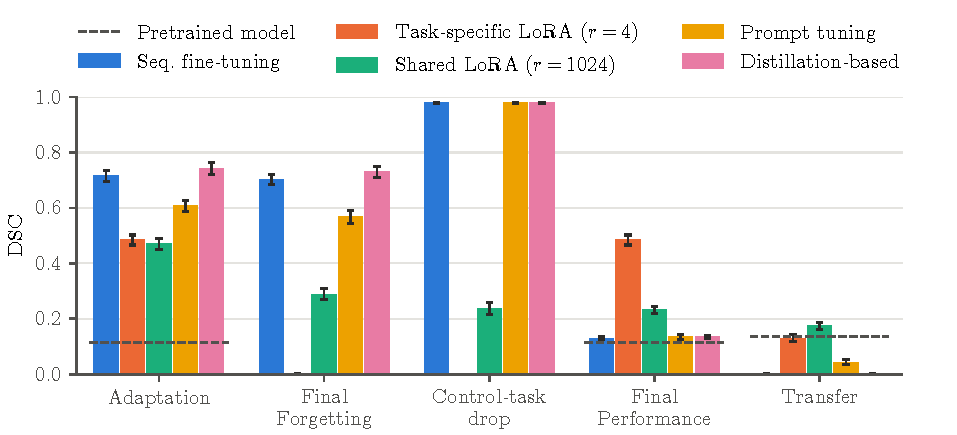
\includegraphics{figures/ch6_main_metrics.pdf}
% CLAUDE-DRAFT
\caption[Metrics of the strategies]{Metrics of the strategies of \cref{tab:ch6_main}, with 95\,\% bootstrap intervals over the test volumes (\cref{subsec:exp-metrics}); joint fine-tuning is shown for the two metrics defined for it.}
\label{fig:ch6_main_metrics}
\end{figure}

% CLAUDE-DRAFT
In the primary metrics, the strategies formed two groups (\cref{tab:ch6_main,fig:ch6_main_metrics}).
The two strategies that update the pretrained weights adapted most and forgot most, whereas the LoRA strategies adapted less and retained much more.
Sequential fine-tuning and the distillation-based strategy reached the highest Adaptation, 0.781 and 0.747, and the highest Final Forgetting, 0.782 and 0.734.
Both lost the control task completely, with a control-task drop of 0.979, and so did joint fine-tuning, although it was trained without a task sequence and with the same total number of updates.
The three LoRA strategies reached an Adaptation of 0.485, 0.471 and 0.472.
Task-specific LoRA keeps every trained task by construction, and shared LoRA reached a Final Forgetting of 0.289 and a control-task drop of 0.237.
With replay, these fell to 0.046 and 0.138, the lowest of the strategies with one parameter set, while the Adaptation of shared LoRA changed by only 0.001 $[-0.002, 0.004]$.
The prompt-tuning strategy reached an Adaptation of 0.580 and a Final Forgetting of 0.510, between the two groups, but its control-task drop of 0.865 is close to that of the first group, although it keeps all pretrained weights frozen.
% source: thesis/tables/cl_metrics.csv (joint: exp_20261022_171655_6a6e9cb5, control-task drop 0.979, moved here from the Final Performance paragraph 2026-11-04); cl_differences.csv (pairs with exp_20261022_171452_a9f4ca56; replay: exp_20261023_014438_55e6abcf - exp_20260926_095539_90e8b4e6); control row of the eval_matrix.csv of each run

% CLAUDE-DRAFT
Within the first group, the distillation-based strategy forgot slightly less than sequential fine-tuning.
Its Final Forgetting was 0.048 lower $[0.039, 0.055]$ at an Adaptation lower by 0.035 $[0.027, 0.041]$, its Final Performance was 0.005 higher $[0.001, 0.009]$, and its control-task drop was the same.
% source: cl_differences.csv, exp_20261022_171452_65011743 - exp_20261022_171452_a9f4ca56
These differences are small compared with the gap to the LoRA strategies and hold for the configuration evaluated here, with an untuned distillation weight $\lambda = 0.01$ (\cref{subsec:method-distillation}).\todo{defense: distillation weight lambda = 0.01 untuned; result holds only for this configuration}

\begin{figure}[tbp] % [p] allowed: too tall to share a page with text
\centering
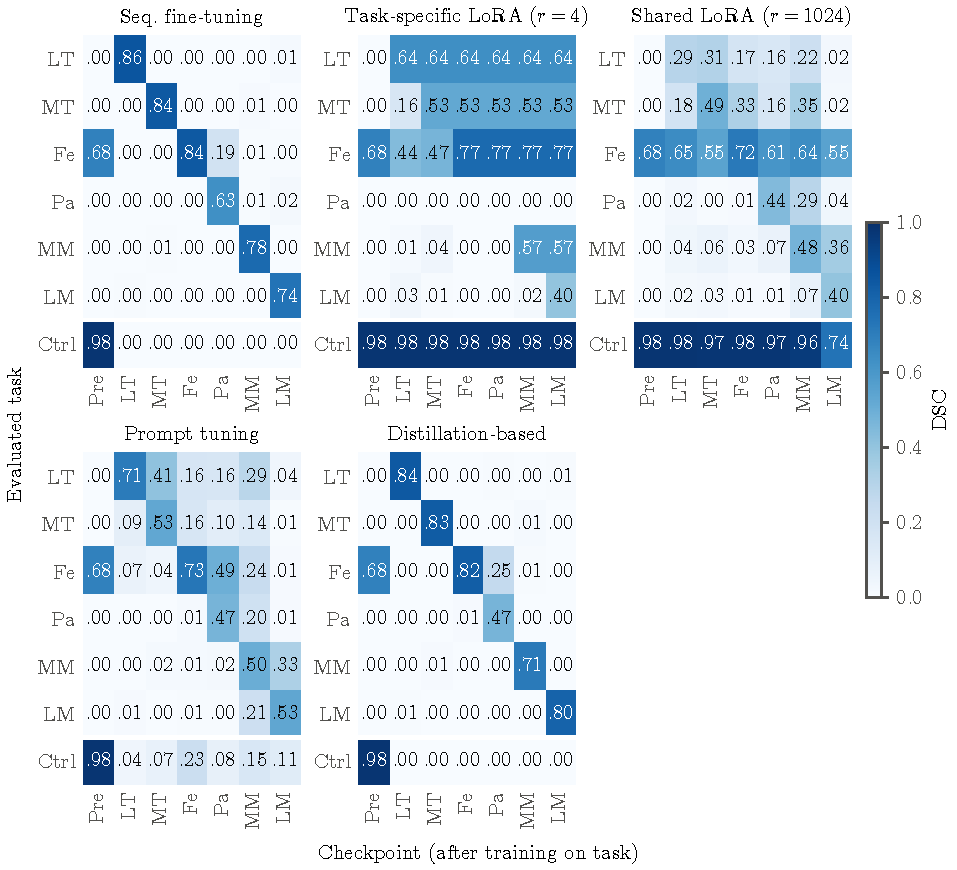
\includegraphics{figures/ch6_main_matrices.pdf}
% CLAUDE-DRAFT
\caption[Evaluation matrices of the strategies]{Evaluation matrices of the strategies: mean \gls{dsc} of each task (rows) at each checkpoint (columns), from the pretrained model (Pre) to the model after the last task. LT, MT: lateral and medial tibial cartilage; Fe: femoral cartilage; Pa: patellar cartilage; MM, LM: medial and lateral meniscus; Ctrl: control task (lung, AeroPath).}
\label{fig:ch6_main_matrices}
\end{figure}

% CLAUDE-DRAFT
The last row of each matrix in \cref{fig:ch6_main_matrices} shows when the control task was lost.
For sequential fine-tuning and the distillation-based strategy, the \gls{dsc} on the lung fell to 0.00 after the first task and did not recover.
For the prompt-tuning strategy, it fell to 0.04 after the first task and then stayed between 0.04 and 0.23.
Shared LoRA, with and without replay, kept the control task at 0.93 or above up to the fifth task and lost most of it in the last task, in which the \gls{dsc} on the lung fell from 0.96 to 0.74 without replay and from 0.93 to 0.84 with it.
Replay thus lowered this drop, although the memory holds no control-task samples.
The memory supplied 55 of the 163 samples of each epoch of the last task, so the adapter was trained on a mixture of structures; whether this is why it lost less of the control task was not tested.
Because the effect arose in the last task, it may also depend on the task order (\cref{sec:exp-task-order}).\todo{defense: replay lowers the control-task drop although the memory holds no control samples; explanation (mixture of structures in the last task) not tested; may depend on the task order}
% source: eval_matrix.csv, row aeropath (Retention), of every run; shared LoRA with and without replay: exp_20261023_014438_55e6abcf and exp_20260926_095539_90e8b4e6; replay memory size 55 and train_batches 163 in task 6 (SLURM log 1848503)
% Replay paragraph merged into this paragraph and l. 144 on 2026-11-04 (author decision: replay is a strategy of the comparison; thesis_notes.md section 1).
% Figure ch6_control_task_main removed 2026-11-04 (author): same data as the Ctrl rows of fig:ch6_main_matrices.

% CLAUDE-DRAFT
After the last task, sequential fine-tuning, the distillation-based and the prompt-tuning strategy segment little beyond the structure trained last.
Their Final Performance of 0.130, 0.135 and 0.155 is only slightly above the 0.114 of the pretrained model, and they lost femoral cartilage, which the pretrained model segmented with a \gls{dsc} of 0.68.
Their \gls{dsc} on it ended at 0.01 or less.
This loss began right after training: for sequential fine-tuning and the distillation-based strategy, the \gls{dsc} of a task at the stages after its training is close to zero.
These are the entries right of the diagonal in \cref{fig:ch6_main_matrices}, and the only one above 0.2 is the \gls{dsc} on femoral cartilage after training on patellar cartilage in the distillation-based strategy, with 0.25.
The prompt-tuning strategy kept more of the earlier tasks, with six entries right of the diagonal above 0.2.
The highest is the \gls{dsc} of 0.49 on femoral cartilage after the model had been trained on patellar cartilage, the next task.
% source: eval_matrix.csv of the five runs (femoral row, last column; entries right of the diagonal > 0.2)
% prompt tuning exp_20261022_180923_7bcbb6cc, rechecked 2026-11-04: six entries > 0.2 (LT after MT 0.407, LT after MM 0.286, Fe after Pa 0.492, Fe after MM 0.235, Pa after MM 0.203, MM after LM 0.327); the draft said seven

% CLAUDE-DRAFT
Of all strategies, task-specific LoRA reached the highest Final Performance, 0.485, because each task keeps its own adapter, although it did not learn patellar cartilage at all (\cref{sec:exp-patellar}).
Shared LoRA with replay followed with 0.450 and shared LoRA with 0.233.
Shared LoRA with replay still segmented every structure at the end, with a \gls{dsc} between 0.38 for medial tibial cartilage and 0.70 for femoral cartilage.
% source: eval_matrix.csv of exp_20261023_014438_55e6abcf, last column (moved from Sec. 6.3, 2026-11-04); control row: at least 0.931 up to the fifth task, 0.842 at the end
Joint fine-tuning reached a Final Performance of 0.852, with a \gls{dsc} between 0.83 for patellar cartilage and 0.87 for femoral cartilage (\cref{sec:app-matrices}).
This is 0.367 more than task-specific LoRA and 0.722 more than sequential fine-tuning, and it shows how far all strategies remain from what the same model reaches when it sees all tasks at once.
% source: cl_metrics.csv; cl_differences.csv (exp_20261022_171655_6a6e9cb5 - main runs); eval_matrix.csv of exp_20261022_171655_6a6e9cb5

% CLAUDE-DRAFT
In Transfer, the LoRA strategies stayed close to the pretrained model, with 0.129, 0.174 and 0.175 against 0.137, whereas sequential fine-tuning, the distillation-based and the prompt-tuning strategy reached only 0.001, 0.002 and 0.043.
Before a task was trained, these three strategies segmented almost none of it.

% CLAUDE-DRAFT
Evaluating the checkpoint with the lowest validation loss instead of the parameters after the last epoch changed the results noticeably only for sequential fine-tuning.
Its Adaptation was 0.059 lower and its Final Forgetting 0.070 lower at the same Final Performance (\cref{sec:app-additional}).
For the distillation-based and the prompt-tuning strategy, the two evaluations differ by at most 0.005.\todo{defense: best-validation checkpoint selected with a noisy validation loss (one random patch per volume); reported only as an additional evaluation}
% source: cl_differences.csv, <run>:best_validation - <run> for the three runs

% Selected-epoch statistics cut 2026-11-04 (author): no research or design question depends on them; data in thesis/tables/selected_epochs.csv

% CLAUDE-DRAFT
No strategy combined the Adaptation of sequential fine-tuning with the retention of the LoRA strategies.
Sequential fine-tuning and the distillation-based strategy lost the control task, and joint fine-tuning lost it as well, without a task sequence.
The prompt-tuning strategy lost most of it although its pretrained weights stay frozen.
The LoRA strategies retained much more at a lower Adaptation, task-specific LoRA by construction.
Task-specific LoRA, the only strategy that uses the task identity, reached the highest Final Performance, and of the strategies with one parameter set, shared LoRA with replay came closest and kept most of the control task.
% The explanation by the training configuration (ten epochs per task) was moved out of this conclusion 2026-11-04 (author): it draws on sec:exp-few-shot and is argued in sec:disc-budget.\todo{defense: one run per strategy; conclusion drafted from Claude's suggestions accepted by the author}

% ---------------------------------------------------------------------
\section{Diagnosis of the Patellar Failure}
\label{sec:exp-patellar}

% CLAUDE-DRAFT
Task-specific LoRA did not learn patellar cartilage in the task sequence: the \gls{dsc} right after training on it was 0.00 with $r = 4$ and with $r = 8$, although shared LoRA with $r = 1024$ reached 0.44 on the same task.
% source: eval_matrix.csv of the task-specific (r = 4, 8) runs and of exp_20260926_095539_90e8b4e6 (shared LoRA r = 1024: 0.4432), patellar row, column after the patellar task; reworded 2026-11-04 when this section moved before the rank experiment
The pretrained model does not segment patellar cartilage either (\gls{dsc} 0.00), and task-specific LoRA starts every task from this model with a new adapter, whereas the shared adapter has already been trained on three tasks when it reaches patellar cartilage.
To find the cause, we trained task-specific LoRA on patellar cartilage alone, first with the settings of the sequence and then with one setting changed at a time: the rank, the learning rate, the training seed and the number of epochs.
Each change tests one explanation: too little capacity, too small steps, an unlucky initialisation or too little training.
The diagnosis does not vary the starting point of the adapter; \cref{sec:disc-budget} discusses its possible role.
\Cref{fig:ch6_patellar_loss} shows the training loss of all runs.
% Table of the patellar diagnosis removed 2026-11-05 (author decision): all its values are in the prose and in the legend of fig:ch6_patellar_loss; configurations of all runs in App. A (matrix captions).

\begin{figure}[tb]
\centering
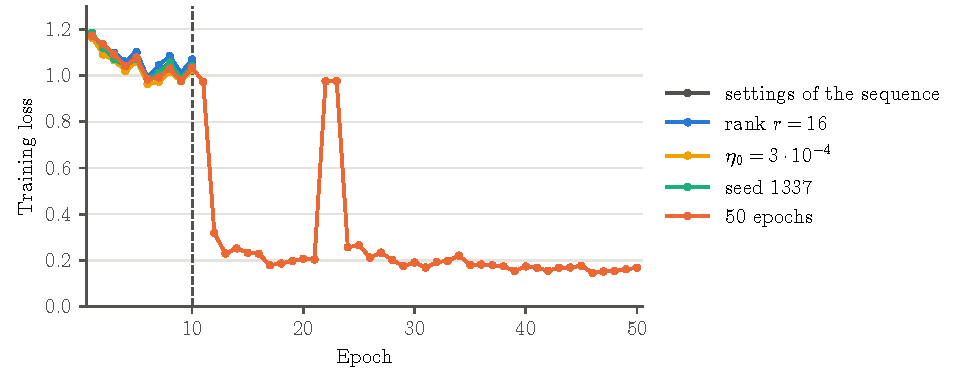
\includegraphics{figures/ch6_patellar_loss.pdf}
% CLAUDE-DRAFT
\caption[Training loss of the patellar diagnosis runs]{Mean training loss per epoch of task-specific LoRA trained on patellar cartilage alone, with the settings of the sequence and with one setting changed per run. Seed: training seed; the data split is the same in all runs. The four runs with 10 epochs lie almost on top of each other. Dashed line: end of training in the task sequence (epoch 10).}
\label{fig:ch6_patellar_loss}
\end{figure}

% CLAUDE-DRAFT
With 10 epochs, every run ended with a \gls{dsc} of 0.000 on the 24 patellar test volumes (95\,\% bootstrap interval $[0.000, 0.000]$), whether with the settings of the sequence, a four times larger rank, a three times larger learning rate or another seed.
With 50 epochs, the same configuration reached 0.839 $[0.811, 0.864]$.
% source: cl_metrics.csv, adaptation and adaptation_ci_low/high of the five Convergence Diagnosis runs (values of the former Table 6.3)
The training loss shows why the runs differ.
In every run, it stayed at about 1.0 during the first ten epochs, close to its value for an empty prediction, for which the Dice term alone is 1.
Only in the 50-epoch run did it drop, from 0.97 at epoch 11 to 0.32 at epoch 12, after which it stayed at about 0.2.
% source: run.log of exp_20260905_220334_6697f1c2 (training loss 1.03 at epoch 10, 0.97 at 11, 0.32 at 12)
At epoch 22, it jumped back to about 1.0 for two epochs and then returned to about 0.2, well before epoch 50, after which the run was evaluated.
% source: run.log of exp_20260905_220334_6697f1c2 (loss per epoch); evaluated checkpoint lora_adapter.pt, saved in after_task after the last epoch (code/src/continual/strategies/lora/task_specific/strategy.py:38; experiment_index.csv eval_checkpoint)

% CLAUDE-DRAFT
Ten epochs were therefore too few for task-specific LoRA to leave the empty prediction on patellar cartilage, and in these runs neither the rank, the learning rate nor the seed was the cause.
The 50-epoch run differs from the others in two ways, however: it has five times as many updates, and its learning rate decays over these 5{,}400 updates, so that at epoch 10 it is still at 80\,\% of $\eta_0$, while in the 10-epoch runs it has reached almost zero.
The experiment does not separate these two effects.
For the comparison of the strategies, the result means that the Adaptation of task-specific LoRA is limited by the training length of the shared configuration and not only by the strategy itself.\todo{defense: shared training configuration (10 epochs) understates task-specific LoRA on patellar cartilage; extra updates and longer LR schedule confounded in the 50-epoch run}

\section{Amount of Labelled Data}
\label{sec:exp-few-shot}
% CLAUDE-DRAFT
This experiment asks how the amount of labelled data affects adaptation and forgetting (\cref{tab:ch6_experiments}).
It uses the few-shot settings and the equal-updates runs of \cref{subsec:exp-data}, with joint fine-tuning on the same $k$ volumes as the reference.
\Cref{tab:ch6_few_shot} gives all metrics, \cref{fig:ch6_few_shot} the main ones, and \cref{sec:app-matrices} the evaluation matrices from which the per-task values below are taken.

\begin{table}[tb]
\centering
% CLAUDE-DRAFT
\caption[Results of the few-shot experiment]{Results of the few-shot experiment (original task order, one run each). Vol.\ (updates): training volumes and updates per task, for joint fine-tuning the total number of updates of its single stage; 108 is the full training split, and 5 (1{,}080) are the equal-updates runs. Mean \gls{dsc}; $\uparrow$/$\downarrow$: higher/lower is better. $^{\dagger}$: zero or near zero by construction (\cref{subsec:method-lora}), not ranked. --: not defined for joint fine-tuning, which trains on all six tasks at once in a single stage.}
\label{tab:ch6_few_shot}
% Generated by scripts/make_results_tables.py from thesis/tables/cl_metrics.csv. Do not edit.
\small\setlength{\tabcolsep}{3pt}
\begin{tabular}{llrrrrr}
\toprule
Strategy & Vol.\ (updates) & Adapt.\,$\uparrow$ & Forg.\,$\downarrow$ & Ctrl.\ drop\,$\downarrow$ & Final\,$\uparrow$ & Transf.\,$\uparrow$ \\
\midrule
Seq. fine-tuning & 5 (50) & 0.545 & 0.382 & 0.010 & 0.227 & 0.092 \\
Seq. fine-tuning & 5 (1{,}080) & 0.712 & 0.714 & 0.979 & 0.117 & 0.023 \\
Seq. fine-tuning & 10 (100) & 0.616 & 0.522 & 0.305 & 0.180 & 0.035 \\
Seq. fine-tuning & 20 (200) & 0.616 & 0.573 & 0.979 & 0.138 & 0.022 \\
Seq. fine-tuning & 108 (1{,}080) & 0.781 & 0.782 & 0.979 & 0.130 & 0.001 \\
\addlinespace
Task-specific LoRA ($r = 4$) & 5 (50) & 0.114 & 0.000$^{\dagger}$ & 0.000$^{\dagger}$ & 0.114 & 0.137 \\
Task-specific LoRA ($r = 4$) & 5 (1{,}080) & 0.429 & 0.000$^{\dagger}$ & 0.000$^{\dagger}$ & 0.429 & 0.059 \\
Task-specific LoRA ($r = 4$) & 10 (100) & 0.115 & 0.000$^{\dagger}$ & 0.000$^{\dagger}$ & 0.115 & 0.137 \\
Task-specific LoRA ($r = 4$) & 20 (200) & 0.116 & 0.000$^{\dagger}$ & 0.000$^{\dagger}$ & 0.116 & 0.138 \\
Task-specific LoRA ($r = 4$) & 108 (1{,}080) & 0.485 & 0.000$^{\dagger}$ & 0.000$^{\dagger}$ & 0.485 & 0.129 \\
\addlinespace
Shared LoRA ($r = 1024$) & 5 (50) & 0.115 & 0.000 & $-$0.001 & 0.115 & 0.137 \\
Shared LoRA ($r = 1024$) & 5 (1{,}080) & 0.438 & 0.296 & 0.334 & 0.192 & 0.175 \\
Shared LoRA ($r = 1024$) & 10 (100) & 0.116 & 0.000 & $-$0.001 & 0.117 & 0.138 \\
Shared LoRA ($r = 1024$) & 20 (200) & 0.140 & $-$0.009 & 0.004 & 0.165 & 0.140 \\
Shared LoRA ($r = 1024$) & 108 (1{,}080) & 0.471 & 0.289 & 0.237 & 0.233 & 0.174 \\
\midrule
Joint fine-tuning & 5 (300 total) & -- & -- & 0.733 & 0.600 & -- \\
Joint fine-tuning & 10 (600 total) & -- & -- & 0.894 & 0.585 & -- \\
Joint fine-tuning & 20 (1{,}200 total) & -- & -- & 0.979 & 0.753 & -- \\
Joint fine-tuning & 108 (6{,}480 total) & -- & -- & 0.979 & 0.852 & -- \\
\midrule
Pretrained model &  & 0.114 & 0.000 & 0.000 & 0.114 & 0.137 \\
\bottomrule
\end{tabular}

\end{table}

\begin{figure}[tb]
\centering
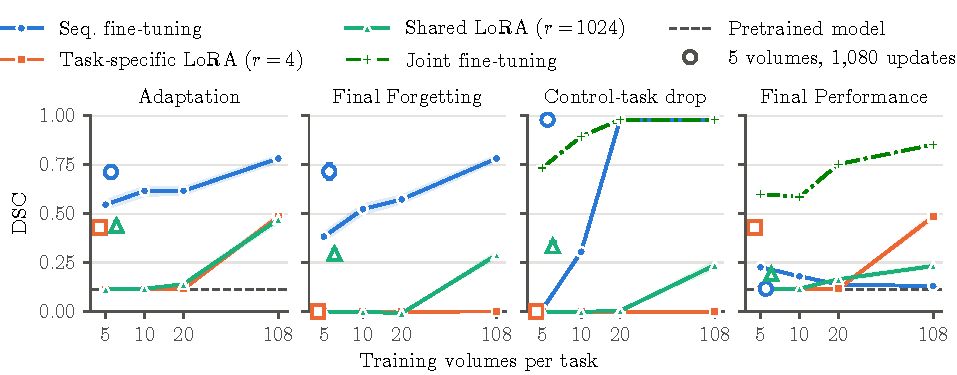
\includegraphics{figures/ch6_few_shot.pdf}
% CLAUDE-DRAFT
\caption[Metrics over the number of training volumes]{Metrics over the number of training volumes per task (logarithmic axis), with 95\,\% bootstrap intervals. Filled markers and solid lines: ten epochs per task; hollow markers at 5 volumes: equal-updates runs with 1{,}080 updates per task, shifted slightly to the side for legibility. Dash-dotted line: joint fine-tuning, shown for the two metrics defined for it. Dashed line: pretrained model.}
\label{fig:ch6_few_shot}
\end{figure}

% CLAUDE-DRAFT
Sequential fine-tuning learned every task in all three few-shot settings, and with fewer volumes it forgot less.
With $k = 5$, its Adaptation was 0.545 instead of 0.781.
Its Final Forgetting, however, was 0.382 instead of 0.782, and it kept the control task, with a drop of 0.010 instead of 0.979.
Its Final Performance was therefore higher than with the full split, 0.227 against 0.130, and it ended with a \gls{dsc} of 0.42 on femoral cartilage, which the full-split run lost.
With $k = 10$ and $k = 20$, Adaptation, Final Forgetting and Final Performance lie between their values with $k = 5$ and with the full split (\cref{tab:ch6_few_shot}).
The control task was lost gradually with $k = 10$ (drop 0.305) and within two tasks with $k = 20$, almost as fast as with the full split, which lost it after the first task.
% source: tables/cl_metrics.csv; cl_differences.csv (few-shot runs - exp_20261022_171452_a9f4ca56); eval_matrix.csv of exp_20261023_212327_a67fb8c9, exp_20261023_234659_f041f82f, exp_20261024_001927_861cfa24

% CLAUDE-DRAFT
With 5 and 10 volumes per task, neither LoRA strategy learned any task, whereas with the full training split they reached an Adaptation of 0.485 and 0.471 (\cref{sec:exp-main}).
Their few-shot Adaptation of 0.114 to 0.116 equals that of the pretrained model (0.114).
The evaluation matrices show why: right after training, every structure except femoral cartilage has a \gls{dsc} of 0.00, and femoral cartilage reaches 0.69 to 0.70, close to the 0.68 of the pretrained model.
Final Forgetting and the control-task drop are therefore about zero for both strategies.
With 20 volumes, task-specific LoRA still did not learn any task, while shared LoRA began to, with an Adaptation of 0.140 and a Final Performance of 0.165.
Its Final Forgetting is slightly negative ($-0.009$), because the structures it began to learn improved further while later tasks were trained.
% source: tables/cl_metrics.csv; eval_matrix.csv of the six few-shot LoRA runs

% CLAUDE-DRAFT
The equal-updates runs separate the number of volumes from the number of updates at $k = 5$.
For the LoRA strategies, the number of updates explains most of the failure: with 1{,}080 updates per task on 5 volumes, task-specific and shared LoRA reached an Adaptation of 0.429 and 0.438, lower by only 0.056 $[0.040, 0.073]$ and 0.032 $[0.025, 0.039]$ than with the full split.
Task-specific LoRA again did not learn patellar cartilage (\gls{dsc} 0.00 right after training), in agreement with \cref{sec:exp-patellar}, where 1{,}080 updates were not enough for this structure.
With more updates, shared LoRA forgot as much as with the full split: its Final Forgetting of 0.296 did not differ from that of the full split (paired interval of the difference $[-0.007, 0.018]$), and its control-task drop of 0.334 was 0.097 higher.
Sequential fine-tuning with 1{,}080 updates on 5 volumes reached an Adaptation of 0.712 instead of 0.545 and forgot as much as with the full split: Final Forgetting 0.714, control-task drop 0.979 and Final Performance 0.117.
% source: cl_metrics.csv; cl_differences.csv (equal-updates runs - k = 5 runs and - full-split runs); eval_matrix.csv of exp_20261023_195739_6044ad8d, exp_20261023_195940_ea9221f2, exp_20261023_200332_9840ab20

% CLAUDE-DRAFT
Joint fine-tuning reached a Final Performance between 0.585 and 0.753 with 5 to 20 volumes per structure, against 0.852 with the full split.
With 5 volumes, it ended 0.373 above sequential fine-tuning with the same total number of updates and 0.170 above task-specific LoRA with equal updates, the best strategy in this setting.
Its control-task drop rose with the total number of updates (\cref{tab:ch6_few_shot}), from 0.733 with $k = 5$ to 0.979 with $k = 20$ and with the full split.
% source: cl_metrics.csv; cl_differences.csv (joint runs); eval_matrix.csv of exp_20261024_002524_abc243ff, exp_20261024_014447_afb34098, exp_20261024_051245_f9067927; full split: train_batches=648 per epoch x 10 epochs (SLURM log voxtell_1848501.out, exp_20261022_171655_6a6e9cb5); seq. FT k = 5: 6 tasks x 50 updates = 300, as joint k = 5

% CLAUDE-DRAFT
With ten epochs per task, sequential fine-tuning was the only one of the three strategies that learned the tasks in the few-shot settings, with 50 to 200 updates per task.
At $k = 5$, the fixed epoch budget explains most of the failure of the LoRA strategies, which learned the tasks with the update count of the full split.
For sequential fine-tuning, the lower forgetting and the kept control task with few volumes are consistent with an effect of the number of updates rather than of the amount of data, so we read its higher Final Performance with 5 volumes as that of a less trained model, not as a benefit of less data.
These conclusions rest on the equal-updates runs at $k = 5$; for $k = 10$ and $k = 20$, the number of volumes and the number of updates remain confounded.
Each configuration was trained once, on one draw of volumes and with a learning rate that was not tuned.\todo{defense: data and updates separated only at k = 5; one support set; one seed; learning rate untuned}

\section{LoRA Rank}
\label{sec:exp-rank}
% CLAUDE-DRAFT
This experiment asks how the rank of the LoRA adapters affects adaptation and forgetting (\cref{tab:ch6_experiments}).
\Cref{tab:ch6_rank} gives all metrics, and \cref{fig:ch6_rank} shows the trend for shared LoRA.

\begin{table}[tb]
\centering
% CLAUDE-DRAFT
\caption[Results of the LoRA rank experiment]{Results of the LoRA rank experiment (full training split, original task order, one run each). Mean \gls{dsc}; $\uparrow$/$\downarrow$: higher/lower is better. Bold: best of the seven ranks of shared LoRA in each column. $^{\dagger}$: zero or near zero by construction (\cref{subsec:method-lora}), not ranked.}
\label{tab:ch6_rank}
% Generated by scripts/make_results_tables.py from thesis/tables/cl_metrics.csv. Do not edit.
\small\setlength{\tabcolsep}{3pt}
\begin{tabular}{llrrrrr}
\toprule
Strategy & Rank $r$ & Adapt.\,$\uparrow$ & Forg.\,$\downarrow$ & Ctrl.\ drop\,$\downarrow$ & Final\,$\uparrow$ & Transf.\,$\uparrow$ \\
\midrule
Task-specific LoRA & 4 & 0.485 & 0.000 & 0.000 & 0.485 & 0.129 \\
Task-specific LoRA & 8 & 0.404 & 0.001 & 0.000 & 0.404 & 0.172 \\
\addlinespace
Shared LoRA & 4 & 0.607 & 0.546 & 0.978 & 0.152 & 0.045 \\
Shared LoRA & 32 & 0.570 & 0.499 & 0.978 & 0.154 & 0.114 \\
Shared LoRA & 128 & 0.524 & 0.384 & 0.957 & 0.204 & 0.170 \\
Shared LoRA & 256 & 0.503 & 0.337 & 0.832 & 0.222 & 0.173 \\
Shared LoRA & 512 & 0.488 & 0.309 & 0.574 & 0.230 & 0.175 \\
Shared LoRA & 1024 & 0.471 & 0.289 & 0.237 & 0.233 & 0.174 \\
Shared LoRA & 2048 & 0.462 & 0.284 & 0.091 & 0.233 & 0.175 \\
\midrule
Pretrained model &  & 0.114 & 0.000 & 0.000 & 0.114 & 0.137 \\
\bottomrule
\end{tabular}

\end{table}

\begin{figure}[tb]
\centering
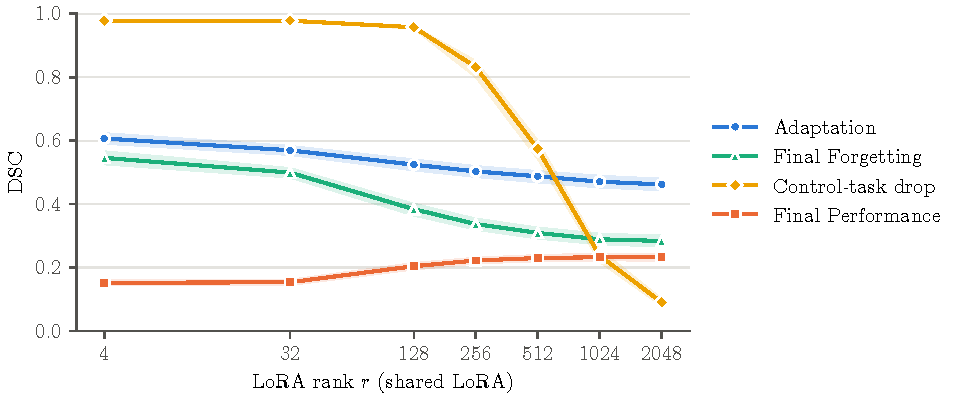
\includegraphics{figures/ch6_rank.pdf}
% CLAUDE-DRAFT
\caption[Metrics of shared LoRA over the rank]{Metrics of shared LoRA over the rank $r$ (logarithmic axis; full training split, original task order, one run per rank). Transfer is given in \cref{tab:ch6_rank}. Shaded bands: 95\,\% bootstrap intervals over the test volumes.}
\label{fig:ch6_rank}
\end{figure}

% CLAUDE-DRAFT
For shared LoRA, Adaptation, Final Forgetting, the control-task drop and Final Performance change monotonically with the rank.
From $r = 4$ to $r = 2048$, Adaptation falls from 0.607 to 0.462, while Final Forgetting falls from 0.546 to 0.284 and the control-task drop from 0.978 to 0.091.
Final Performance rises from 0.152 at $r = 4$ to 0.230 at $r = 512$ and hardly changes at higher ranks.
Transfer rises from 0.045 at $r = 4$ to 0.170 at $r = 128$ and stays between 0.170 and 0.175 at higher ranks.
The control-task drop changes most: up to $r = 32$, the lung is no longer segmented at all after the last task, and only the two highest ranks keep most of it.
% source: thesis/tables/cl_metrics.csv; c_T from the eval_matrix.csv of each run (0.00 at r = 4 and 32, 0.74 at 1024, 0.89 at 2048)

% CLAUDE-DRAFT
The evaluation matrices show which tasks drive these trends (\cref{sec:app-matrices}).
The gain in Final Performance comes from femoral cartilage, which the pretrained model already segments with a \gls{dsc} of 0.68.
It is lost by the end of the sequence at $r = 4$ and $r = 32$ but kept at 0.54 to 0.55 from $r = 512$ on, whereas lateral tibial, medial tibial and patellar cartilage end below 0.06 at every rank and the two menisci between 0.35 and 0.55.
Lateral tibial cartilage, the first task, accounts for the largest share of the fall in Adaptation.
Its \gls{dsc} right after training falls from 0.69 at $r = 4$ to 0.28 at $r = 2048$, whereas that of each other task falls by at most 0.17.
% source: eval_matrix.csv of the shared-LoRA rank runs (diagonal and last column); last column checked 2026-11-05: femoral 0.00, 0.02, 0.36, 0.48, 0.54, 0.55, 0.55 (r = 4 ... 2048); LT, MT, Pa <= 0.05; MM 0.35-0.38, LM 0.55 -> 0.39. The draft said "two structures"; only femoral cartilage gains

% CLAUDE-DRAFT
In shared LoRA, $\alpha = 32$ is the same for all ranks, so the scaling factor $\gamma_r = \alpha / \sqrt{r}$ (\cref{subsec:method-lora}) falls from 16 at $r = 4$ to 0.71 at $r = 2048$ (\cref{tab:app-strategy-params}).
The rank and the scaling factor therefore change together, so this experiment does not separate the effect of the adapter's capacity from that of its scale.\todo{defense: rank and $\gamma_r$ confounded in the shared-LoRA rank ablation (alpha fixed); rsLoRA intends rank-stable training, not tested here}

% CLAUDE-DRAFT
For task-specific LoRA, $r = 8$ reached a lower Adaptation than $r = 4$ (0.404 against 0.485).
The difference comes from lateral tibial cartilage (0.52 against 0.64) and lateral meniscus (0.12 against 0.40), while the other tasks differ by at most 0.05.
% source: eval_matrix.csv of the two task-specific LoRA runs
Each rank was trained once, so we cannot determine whether such differences between single tasks come from the rank or from the training randomness.

% CLAUDE-DRAFT
For shared LoRA with fixed $\alpha$, the rank sets a trade-off between adaptation and retention: higher ranks forget less, both of the trained tasks and of the control task, at a cost in Adaptation.
Why higher ranks retain more remains open.
For the comparison of the strategies, we use $r = 1024$ for shared LoRA.
It has half the trainable parameters of $r = 2048$ (50.3 against 100.7 million) and the same Final Performance, and its Adaptation and Final Forgetting differ by less than 0.01.
The control-task drop, however, still falls from 0.237 to 0.091 between the two ranks, so the comparison of the strategies understates how much of the control task shared LoRA can keep.\todo{defense: r = 1024 chosen for parameter count and saturation of Adaptation, Final Forgetting and Final Performance; control-task drop not saturated}
For task-specific LoRA, doubling the rank brought no gain in this run, so we use $r = 4$.

\section{Task Order}
\label{sec:exp-task-order}
% CLAUDE-DRAFT
This experiment asks whether the results depend on the order in which the structures are learned, for the three strategies trained in both task orders (\cref{subsec:exp-data}).
\Cref{tab:ch6_task_order} gives all metrics, \cref{fig:ch6_task_order} the main ones, and \cref{sec:app-matrices} the evaluation matrices from which the per-task values below are taken.

\begin{table}[tb]
\centering
% CLAUDE-DRAFT
\caption[Results of the task-order experiment]{Results of the task-order experiment (full training split, one run each). The pretrained-model reference is computed for each task order. Mean \gls{dsc}; $\uparrow$/$\downarrow$: higher/lower is better. $^{\dagger}$: zero or near zero by construction (\cref{subsec:method-lora}), not ranked.}
\label{tab:ch6_task_order}
% Generated by scripts/make_results_tables.py from thesis/tables/cl_metrics.csv. Do not edit.
\small\setlength{\tabcolsep}{3pt}
\begin{tabular}{llrrrrr}
\toprule
Strategy & Task order & Adapt.\,$\uparrow$ & Forg.\,$\downarrow$ & Ctrl.\ drop\,$\downarrow$ & Final\,$\uparrow$ & Transf.\,$\uparrow$ \\
\midrule
Seq. fine-tuning & Original & 0.781 & 0.782 & 0.979 & 0.130 & 0.001 \\
Seq. fine-tuning & Reverse & 0.784 & 0.780 & 0.979 & 0.134 & 0.014 \\
\addlinespace
Task-specific LoRA ($r=4$) & Original & 0.485 & 0.000$^{\dagger}$ & 0.000$^{\dagger}$ & 0.485 & 0.129 \\
Task-specific LoRA ($r=4$) & Reverse & 0.478 & 0.002$^{\dagger}$ & 0.000$^{\dagger}$ & 0.478 & 0.132 \\
\addlinespace
Shared LoRA ($r=1024$) & Original & 0.471 & 0.289 & 0.237 & 0.233 & 0.174 \\
Shared LoRA ($r=1024$) & Reverse & 0.439 & 0.124 & 0.067 & 0.345 & 0.169 \\
\midrule
Pretrained model & Original & 0.114 & 0.000 & 0.000 & 0.114 & 0.137 \\
Pretrained model & Reverse & 0.114 & 0.000 & 0.000 & 0.114 & 0.137 \\
\bottomrule
\end{tabular}

\end{table}

\begin{figure}[tb]
\centering
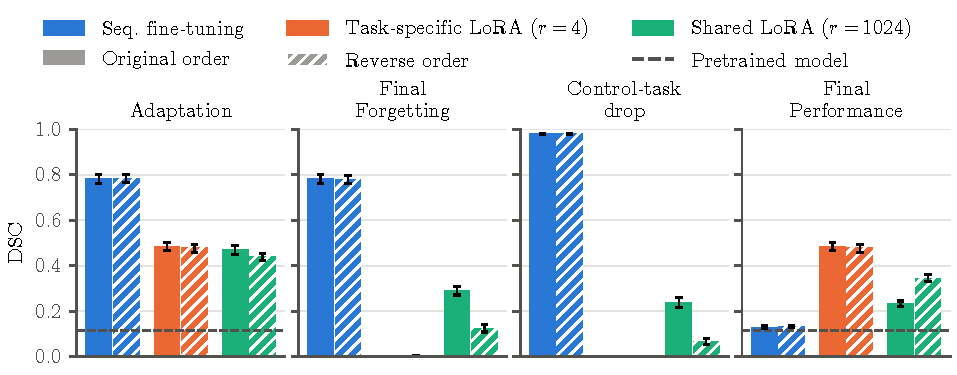
\includegraphics{figures/ch6_task_order.pdf}
% CLAUDE-DRAFT
\caption[Metrics in the original and the reverse task order]{Metrics in the original (plain bars) and the reverse task order (hatched bars), full training split, one run each, with 95\,\% bootstrap intervals. Dashed line: pretrained model.}
\label{fig:ch6_task_order}
\end{figure}

% CLAUDE-DRAFT
For sequential fine-tuning, no effect of the task order can be detected.
In the reverse order, Adaptation was 0.003 higher $[-0.005, 0.010]$, Final Forgetting 0.002 lower $[-0.005, 0.009]$ and Final Performance 0.004 higher $[-0.002, 0.010]$.
In both orders, sequential fine-tuning forgot almost all earlier tasks (Final Forgetting 0.782 and 0.780) and lost the control task after the first task (\gls{dsc} 0.00 in both).
Only Transfer differed, 0.014 instead of 0.001 ($+0.013$, $[0.012, 0.014]$).
This difference is small and comes from the order itself: in the reverse order, femoral cartilage is trained after patellar cartilage and reached a \gls{dsc} of 0.19 before its own task.
% source: tables/cl_metrics.csv; cl_differences.csv (exp_20261022_171520_2dba6ff1 - exp_20261022_171452_a9f4ca56); eval_matrix.csv of both runs

% CLAUDE-DRAFT
For task-specific LoRA, the task order changes neither the data nor the settings of a task: every task starts from the pretrained model with a new adapter (\cref{subsec:method-lora}), and the random seed is reset at the start of every task.
Only the random initialisation of each adapter differs between the two orders, because the adapter is created before the seed is reset, and the training allows non-deterministic GPU operations.
% source: code/src/continual/strategies/base.py (configure_engine before trainer.fit), training/utils.py (seed_everything, use_deterministic_algorithms with warn_only=True)
The two runs therefore show how much a single run varies with its initialisation.
Four of the six tasks reached the same \gls{dsc} within 0.001.
Lateral tibial cartilage reached 0.64 in the original and 0.65 in the reverse order, and lateral meniscus 0.40 and 0.34, so that Adaptation differs by 0.006 (0.485 against 0.478).
The paired bootstrap interval of this difference, $[0.004, 0.008]$, does not contain zero, although the difference comes only from the initialisation and the non-determinism of training.
This illustrates the limit stated in \cref{subsec:exp-metrics}: an interval that excludes zero shows that two trained models differ, not that the factor varied between them caused the difference, and differences of this size between single runs can arise from training randomness alone.\todo{defense: paired intervals exclude zero for a pure re-initialisation difference (task-specific LoRA original vs reverse); training variability not covered}
% source: thesis/tables/cl_differences.csv (adaptation, TIL-LoRA r = 4 original - reverse)

% CLAUDE-DRAFT
For shared LoRA, the reverse order led to better retention.
Final Forgetting was 0.124 instead of 0.289 and the control-task drop 0.067 instead of 0.237, and Final Performance rose from 0.233 to 0.345, while Adaptation was 0.032 lower $[0.022, 0.042]$ (0.439 against 0.471).
% source: cl_differences.csv, CIL-LoRA r = 1024 original - reverse: adaptation +0.032 [0.022, 0.042], final_forgetting +0.165 [0.145, 0.183], control_drop +0.170 [0.162, 0.178], final_performance -0.112 [-0.124, -0.101]
At the end of the reverse sequence, every structure is still segmented to some degree, from 0.13 for lateral meniscus to 0.51 for lateral tibial cartilage, whereas in the original order three of the six structures end below 0.05.
Transfer is about the same in both orders (0.169 and 0.174).
% source: eval_matrix.csv of the two shared-LoRA runs (r = 1024)

% CLAUDE-DRAFT
For shared LoRA in the original order, most of the control-task drop and of the forgetting arose in the last step.
Training on lateral meniscus lowered the \gls{dsc} on the control task from 0.96 to 0.74 (\cref{sec:exp-main}).
In the same step, lateral tibial, medial tibial and patellar cartilage fell from between 0.22 and 0.35 to 0.04 or less.
In the reverse order, the last task, lateral tibial cartilage, lowered the \gls{dsc} on the control task only from 0.97 to 0.91, and that on femoral cartilage, which lost most in this step, from 0.65 to 0.50.
% source: eval_matrix.csv of exp_20260926_095539_90e8b4e6 (original) and exp_20260930_101141_5d80eb69 (reverse), last two columns (original, LM step: LT 0.22 -> 0.02, MT 0.35 -> 0.02, Pa 0.29 -> 0.04)
Whether lateral meniscus causes this loss as a structure or through its position at the end of the sequence cannot be separated with two orders.

% Moved 2026-11-05 (author decision): the first-task observation now follows the retention block and precedes the training-loss paragraph that explains it.
% CLAUDE-DRAFT
In both orders, shared LoRA learned the first task poorly.
Lateral tibial cartilage, the first task of the original order, reached 0.29 right after training, but 0.51 when it was trained last in the reverse order.
Lateral meniscus, the first task of the reverse order, reached 0.01, but 0.40 when it was trained last in the original order.
Sequential fine-tuning, by contrast, learned the first task well in both orders, lateral tibial cartilage with 0.86 and lateral meniscus with 0.83.
% source: eval_matrix.csv of the two shared-LoRA runs (r = 1024) and of the two sequential fine-tuning runs (exp_20261022_171452_a9f4ca56, exp_20261022_171520_2dba6ff1), diagonal

% CLAUDE-DRAFT
The training loss of shared LoRA with $r = 1024$ (\cref{fig:app-shared-loss}) shows how the first task differs from the later ones.
On the first task, the loss started at about 1.0, its value for an empty prediction, and fell slowly: in the original order to 0.69 after ten epochs, in the reverse order only to 0.96.
On the second task, it started much lower, at 0.81 in the original and 0.86 in the reverse order in the first epoch, and fell to 0.56 in both orders, although in the reverse order the first task was hardly learned at all.
For shared LoRA with $r = 4$ in the original order, by contrast, the loss of the first task fell to 0.74 within three epochs and to 0.38 after ten, in line with the higher \gls{dsc} of the first task at low ranks (\cref{sec:exp-rank}).
% source: run.log of the shared-LoRA runs (r = 4 and r = 1024, original and reverse), "Training Loss" per epoch

% CLAUDE-DRAFT
For sequential fine-tuning, the task order changed only Transfer, by 0.013, and it forgot almost everything in both orders.
For task-specific LoRA, the task order has no effect beyond the variation between two runs, as its design implies.
For shared LoRA, the task order has a strong effect: in the reverse order, the adapter retained more of the earlier tasks and of the control task, at a lower Adaptation.
With two orders, we cannot determine which property of the order causes this difference in retention.
In both orders, the first task was learned poorly, and the training loss shows that its adapter had not left its initial state after ten epochs; a possible explanation, which connects this observation with the rank, patellar and few-shot experiments, is discussed in \cref{sec:disc-budget}.

% ---------------------------------------------------------------------
\section{Weight Ensemble and Gradient Scaling}
\label{sec:exp-components}
% Split from Sec. 6.2 on 2026-11-02 (author decision; reverses the 2026-10-24 decision, thesis_notes.md section 1).
% Narrowed 2026-11-04 (author decision): replay moved to Sec. 6.2; title changed from "Components of the Strategies"; label kept.
% CLAUDE-DRAFT
This experiment asks how the weight ensemble of the distillation-based strategy and the per-task gradient scaling of the prompt-tuning strategy affect adaptation and forgetting (\cref{tab:ch6_experiments}).
Both components are adopted from the published methods, ZSCL and CPE-CLIP, and each is compared with the same strategy without it.
The weight ensemble is evaluated in the same run as the student, and gradient scaling is compared against an earlier run without it.
\Cref{tab:ch6_components} in \cref{sec:app-additional} gives the metrics of these evaluations, and \cref{tab:ch6_main} gives those after the last epoch.

% CLAUDE-DRAFT
The weight ensemble of the distillation-based strategy halved the Adaptation of the student, from 0.747 to 0.376, lowered the Final Performance by 0.011 $[0.007, 0.017]$ and left the control-task drop unchanged.
Its Final Forgetting of 0.354, against 0.734 for the student, is lower only because the ensemble learned less in the first place.
On the diagonal of its evaluation matrix (\cref{tab:app-we-matrix}), the \gls{dsc} fell from 0.83 on the first task to 0.22 on the fourth and to 0.00 on the last two.
A possible explanation follows from the definition of the ensemble as the equally weighted mean of $\theta_0$ and all snapshots, with 100 snapshots per task (\cref{subsec:method-distillation}).
After task~$t$, the snapshots of that task make up only about $1/t$ of the ensemble, so it follows each later task less.
The ensemble also could not protect the control task, because the student had already lost it after the first task (\gls{dsc} 0.00), and the ensemble averages such states.
Our ensemble differs from that of ZSCL in its update interval, in not being restarted at each task and in the distillation without a reference dataset (\cref{subsec:method-distillation}), so these results hold for our configuration only.\todo{defense: weight ensemble not restarted per task and not carried forward (unlike ZSCL's code), interval of 10, no reference dataset; explanation of the low Adaptation (weights of late snapshots) not tested}
% source: cl_differences.csv, exp_20261022_171452_65011743:weight_ensemble - exp_20261022_171452_65011743; diagonal of evaluations/weight_ensemble/eval_matrix.csv; 100 ensemble updates per task (10 per epoch, thesis_notes.md §2)

% CLAUDE-DRAFT
The per-task gradient scaling of the prompt-tuning strategy lowered its forgetting at a small cost in Adaptation.
Both runs are compared at the checkpoint with the lowest validation loss, because the run without scaling was evaluated only there.
With scaling, Final Forgetting was 0.063 lower, the control-task drop 0.117 lower and Final Performance 0.020 higher $[0.014, 0.025]$, at an Adaptation lower by 0.032 $[0.025, 0.040]$.
Without scaling, the \gls{dsc} on the lung fell to 0.02 after the second task and to 0.00 at the end.
With scaling, it stayed between 0.04 and 0.23 from the first task on.
Scaling down the gradients in later tasks thus traded a little adaptation for retention, but it did not keep the control task.
% source: cl_differences.csv, exp_20261022_180923_7bcbb6cc:best_validation - exp_20260816_161201_b39ea60e; control rows of both runs (best_validation/eval_matrix.csv: 0.042-0.226, checked 2026-11-04)

% Conclusion suggested by Claude and accepted by the author (2026-11-04), replacing that of 2026-11-02 after replay moved to Sec. 6.2.
% CLAUDE-DRAFT
Of the two components, only the gradient scaling moved its strategy towards retention, at a small cost in Adaptation.
Neither kept the control task.
The student of the distillation-based strategy had already lost it after the first task, and the prompt-tuning strategy lost most of it with scaling as well.
Both components differ from their published form (\cref{sec:method-strategies}), and each was tested in one run and in the original task order, so these results hold for our configuration only.\todo{defense: components tested once each, one strategy, one task order; scaling compared at best-validation checkpoints against an earlier run}

\section{Computational Cost}
\label{sec:exp-compute}
% CLAUDE-DRAFT
This section reports the measured cost of the strategies, which complements the complexity analysis of \cref{sec:method-complexity}.
\Cref{tab:ch6_compute} gives, for the runs of the comparison of the strategies, the number of trainable parameters, the time per epoch, the total time of the run, the evaluation time per volume and the peak GPU memory, all taken from the logs of the runs.
% source: thesis/tables/compute.csv (scripts/make_compute_table.py)

\begin{table}[tb]
\centering
% CLAUDE-DRAFT
\caption[Measured cost of the strategies]{Measured cost of the strategies in the comparison (full training split, original task order, one NVIDIA A100 40\,GB). Trainable param.: parameters set as trainable, in millions; of the 440.03 million of sequential fine-tuning and the distillation-based strategy, 339.29 million receive gradients (\cref{sec:method-adaptation}). Epoch: mean wall-clock time of one training epoch including validation. Wall-clock: total time of all jobs of the run, including the evaluation of the protocol and restarts after the 24-hour limit. Evaluation: median time per test volume, including data loading and text encoding. Peak GPU mem.: maximum over all jobs of the run.}
\label{tab:ch6_compute}
% Generated by scripts/make_compute_table.py from the experiment logs. Do not edit.
\small\setlength{\tabcolsep}{4pt}
\begin{tabular}{lrrrrr}
\toprule
Strategy & Trainable & Epoch & Wall-clock & Evaluation & Peak GPU \\
 & param.\ (M) & (min) & (h) & (s/volume) & mem.\ (GiB) \\
\midrule
Seq. fine-tuning & 440.03 & 26.8 & 32.5 & 8.8 & 31.4 \\
Task-specific LoRA ($r=4$) & 0.20 & 18.1 & 20.8 & 7.9 & 20.3 \\
Shared LoRA ($r=1024$) & 50.33 & 19.8 & 22.6 & 8.5 & 20.6 \\
Prompt tuning & 12.60 & 18.9 & 24.0 & 8.0 & 20.3 \\
Distillation-based & 440.03 & 37.1 & 47.1 & 8.7 & 37.9 \\
\bottomrule
\end{tabular}

\end{table}

% CLAUDE-DRAFT
The two LoRA strategies and the prompt-tuning strategy took 18.1 to 19.8 minutes per epoch, 26 to 33\,\% less than sequential fine-tuning with 26.8 minutes, which agrees with their backward pass ending at the prompt decoder instead of reaching the image encoder.
The earlier run of sequential fine-tuning with the same configuration took 23.7 minutes per epoch; we did not investigate this difference on the shared cluster.
The distillation-based strategy took 37.1 minutes per epoch, 1.4 times as long as sequential fine-tuning, because every iteration adds a forward pass of the teacher and its transfer from CPU to GPU memory.
A complete run, including its evaluations, took 20.8 and 22.6 hours for the two LoRA strategies, 24.0 hours for the prompt-tuning strategy, 32.5 hours for sequential fine-tuning and 47.1 hours for the distillation-based strategy, whose run includes three evaluations; all but the LoRA runs needed a second job.
% source: compute.csv, columns epoch_minutes, job_hours, slurm_jobs; exp_20260816_155351_cfa776e7 for the earlier run
The peak GPU memory was 20.3 to 20.6\,GiB for the parameter-efficient strategies, 31.4\,GiB for sequential fine-tuning and 37.9\,GiB for the distillation-based strategy, close to the 40\,GB of the GPU.

% CLAUDE-DRAFT
For shared LoRA, the number of trainable parameters grows linearly with the rank, from 0.2 million at $r = 4$ to 100.7 million at $r = 2048$, while the time per epoch stays between 18.0 and 21.0 minutes and the peak memory between 20.4 and 20.8\,GiB.
Replay increased the mean time per epoch of shared LoRA with $r = 1024$ from 19.8 to 26.4 minutes, because the replayed samples, up to 55 in the last task, add iterations to every epoch.
In the few-shot settings, an epoch of sequential fine-tuning took 3.1 to 6.5 minutes for $k = 5$ to $k = 20$, of which the validation on the 23 validation volumes, which does not depend on~$k$, is a large part.
The equal-updates runs, with 216 short epochs per task, took 18.4 to 24.3 hours of training, about as long as the full-data runs of the same strategies.
Joint fine-tuning took about 2.3 hours per epoch with its 648 training volumes, measured over the nine epochs whose end was logged, and its four jobs took 50.0 hours in total.
% source: compute.csv (replay, few-shot, equal-updates and joint runs); joint: epoch_minutes 138.0 over 9 epochs (epoch 10 has no completion line: the job resumed after its last batch, SLURM 1850677), job_hours 50.0
After $T$ tasks, task-specific LoRA stores six adapters of 0.2 million parameters each, which is negligible compared with the model.
% source: compute.csv (rank, replay and few-shot runs)

% CLAUDE-DRAFT
Evaluation took 7.7 to 8.8 seconds per volume in the runs of the task sequence, so that the 1{,}036 volume inferences of one evaluation of the protocol (\cref{sec:method-complexity}) took about 2.2 to 2.5 hours.
The forward pass has the same cost for all strategies; the measured times also include loading the volumes and encoding the text prompts, and we did not investigate the differences between runs.

% CLAUDE-DRAFT
All strategies fit on a single 40\,GB GPU.
The parameter-efficient strategies are the cheapest to train, with a quarter to a third less time per epoch and about a third less memory than sequential fine-tuning, and the distillation-based strategy is the most expensive in both time and memory.
At inference, the strategies cost the same.
